\section{The case $[2 \times 3, 6]_4$}
\begin{lemma}
  Let $p = (p_3, p_4, p_5, \dots, p_n)$ be a given sequence satisfying equation \ref{eq_valence_4} as well as $p_4 \leq 3$, $p_5 \leq 3$ and $3 \mid 2 \sum_{k=3}^{n} p_k - 4$. Then there exists $r \in \nats$ for which $p + r [2 \times 3, 6]_3$ is $4$-realizable.

  All the requirements in the statement will help utilizing Eberhards Theorem \ref{thm_eberhard}(\ref{thm_eberhard_3}). The conditions $p_4 \leq 3$, $p_5 \leq 3$ deal with different sign of curvatures when having valence $3$ and $4$ (note that quadrangles and pentagons have positive curvature in the case of $3$-valence but zero or negative curvature in the other case), while the condition $p_4 \leq 3$, $p_5 \leq 3$ is necessary to keep the number of triangles natural. 
  \begin{proof}
    One can restate \ref{eq_valence_4} to a form looking more like \ref{eq_valence_3}:
    \begin{align*}
      & \sum_{k=3}^n \left( 4 - k \right) p_k = 8 \\
      \implies & \sum_{k=3}^n \left( 6 - k \right) p_k - \left(2 \sum_{k=3}^n  p_k - 4 \right) = 12
    \end{align*}
    Let $r_3 := (2 \sum_{k=3}^{n} p_k - 4)/3$. From
    \begin{align*}
      3 r_3 &= 2 \sum_{k=3}^{n} p_k - 4 =  2 p_3 + 2 p_4 + 2 p_5 + \sum_{k=6}^{n} p_k - 4\\
      \implies r_3 &= 2 p_4 + 2 p_5 - 4 + \sum_{k=6}^{n} p_k \leq 8 + 2 \sum_{k=6}^{n} p_k \leq 8 + \sum_{k=4}^{n} (k - 4) p_k = p_3
    \end{align*}
    follows, that $p_3' := p_3 - r_3 \geq 0$ and setting $p_k' := p_k$, $(k \geq 4)$ the resulting sequence $p'$ suffices \ref{eq_valence_3}. Using \ref{thm_eberhard}(\ref{thm_eberhard_3}) one get a $3$-realization $P'$ of $p'$. Inserting in $P'$ an hexagon for every edge and four triangles for every vertex as seen in the following figure one can construct a $4$-realization of some sequence $p''$.
    \begin{figure}[htpp]
      \centering
      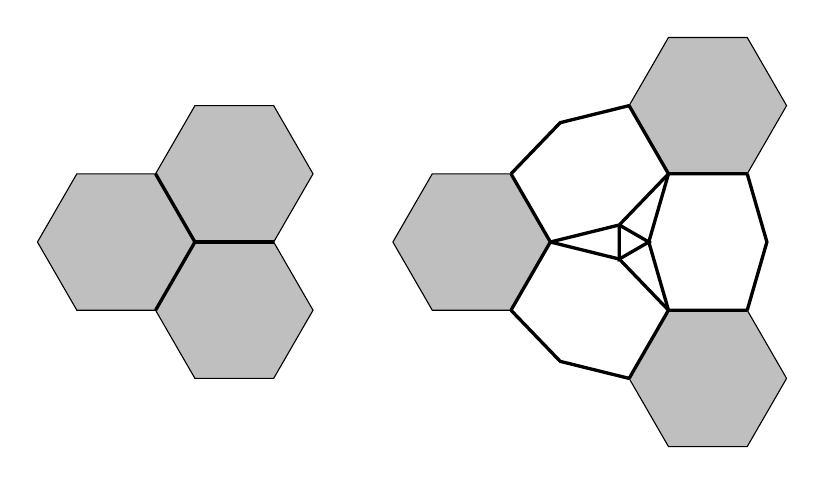
\begin{tikzpicture}
        \matrix (m) [ column sep=1cm] {
          \begin{scope}[xscale=1.0, yscale=0.866]
            \filldraw[fill=gray!50!white] (0, 1) -- ++(0.5, -1) -- ++(1, 0) -- ++(0.5, 1) -- ++(-0.5, 1) -- ++(-1, 0) -- ++(-0.5, -1);
            \filldraw[fill=gray!50!white] (1.5, 0) -- ++(0.5, -1) -- ++(1, 0) -- ++(0.5, 1) -- ++(-0.5, 1) -- ++(-1, 0) -- ++(-0.5, -1);
            \filldraw[fill=gray!50!white] (1.5, 2) -- ++(0.5, -1) -- ++(1, 0) -- ++(0.5, 1) -- ++(-0.5, 1) -- ++(-1, 0) -- ++(-0.5, -1);
            \draw[very thick] (1.5, 0) -- ++(0.5, 1) -- ++(-0.5, 1);
            \draw[very thick] (2, 1) -- ++(1, 0);
          \end{scope}
          &
          \begin{scope}[xscale=1.0, yscale=0.866] 
            \filldraw[fill=gray!50!white] (-1.5, 1) -- ++(0.5, -1) -- ++(1, 0) -- ++(0.5, 1) -- ++(-0.5, 1) -- ++(-1, 0) -- ++(-0.5, -1);
            \filldraw[fill=gray!50!white] (1.5, -1) -- ++(0.5, -1) -- ++(1, 0) -- ++(0.5, 1) -- ++(-0.5, 1) -- ++(-1, 0) -- ++(-0.5, -1);
            \filldraw[fill=gray!50!white] (1.5, 3) -- ++(0.5, -1) -- ++(1, 0) -- ++(0.5, 1) -- ++(-0.5, 1) -- ++(-1, 0) -- ++(-0.5, -1);
            \draw[very thick] (0, 0) -- ++(0.5, 1) -- ++(-0.5, 1);
            \draw[very thick] (1.5, -1) -- ++(0.5, 1) -- ++(1, 0);
            \draw[very thick] (1.5, 3) -- ++(0.5, -1) -- ++(1, 0);

            \draw[very thick] (0.5, 1) -- (1.375, 1.25) -- (2, 2);
            \draw[very thick] (0.5, 1) -- (1.375, 0.75) -- (2, 0);
            \draw[very thick] (2, 0) -- (1.75, 1) -- (2, 2);
            \draw[very thick] (1.375, 1.25) -- (1.375, 0.75) -- (1.75, 1) -- (1.375, 1.25);
            \draw[very thick] (0, 2) -- (0.625, 2.75) -- (1.5, 3);
            \draw[very thick] (0, 0) -- (0.625, -0.75) -- (1.5, -1);
            \draw[very thick] (3, 0) -- (3.25, 1) -- (3, 2);

          \end{scope};
          \\
        };
      \end{tikzpicture}
    \end{figure}
    $p''$ coincides with $p$ for every entry but $3$ and $6$. They both comply with \ref{eq_valence_4}, therefore
    \begin{align*}
      & \sum_{k=3}^n \left( 4 - k \right) p''_k  - \sum_{k=3}^n \left( 4 - k \right) p_k = 0 \\
      \implies & 2(p''_3 - p_3) = p''_6 - p_6
    \end{align*}
    and $p'' = p + (p''_6 - p_6)[2 \times 3, 6]_4$ is $4$-realizable, which finishes the proof.
  \end{proof}
\end{lemma}

\begin{lemma}
  Let $p = (p_3, p_4, p_5, \dots, p_n)$ and $q = (q_3, q_4, q_5, \dots, q_m)$ be two sequence which can be realized up to a scalar multiple of $[2 \times 3, 6]_4$, then the sequence $p + q - [8 \times 3]_4$ is $4$-realizable, also up to some scalar factor.
  \begin{proof}
    Let $P$ and $Q$ by the $4$-realizations of $p$ and $q$. By extruding every face of both realizations as seen below, adding multiple hexagons and triangles around each one, a much larger complex is build.
    \begin{figure}[htpp]
      \centering
      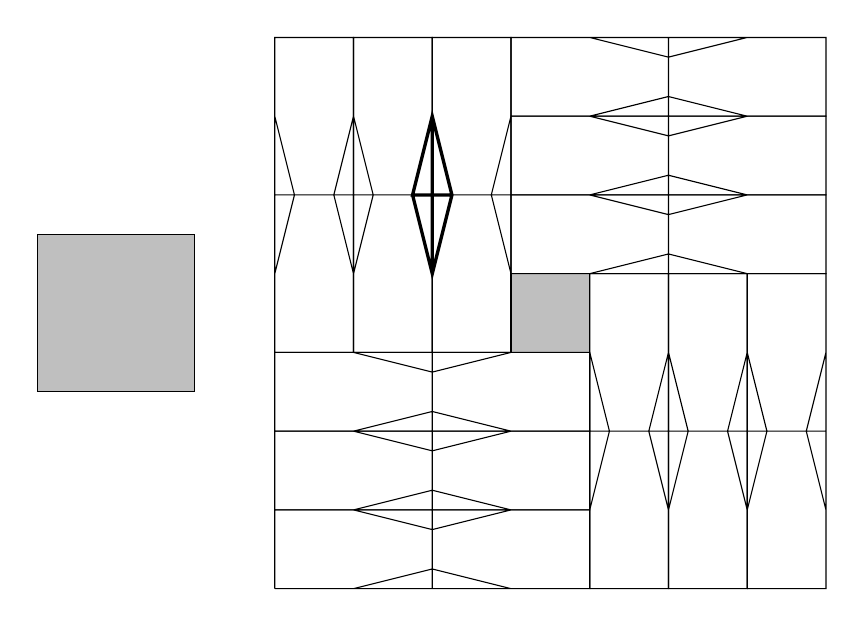
\begin{tikzpicture}
        \matrix (m) [ column sep=1cm] {
          \begin{scope}
            \filldraw[fill=gray!50!white] (-1, -1) -- (-1, 1) -- (1, 1) -- (1, -1) -- (-1, -1);
            %\draw[very thick] (-1, -1) -- (-1, 1) -- (1, 1) -- (1, -1) -- (-1, -1);
          \end{scope}
          &
          \begin{scope}[scale=0.5] 
            \filldraw[fill=gray!50!white] (-1, -1) -- (-1, 1) -- (1, 1) -- (1, -1) -- (-1, -1);
            %\draw[very thick] (-1, -1) -- (-1, 1) -- (1, 1) -- (1, -1) -- (-1, -1);
 -2) ++(-1, 0) -- ++(-0.5, 2);
            \draw (-7, -1) -- ++(2, 0) -- ++(0, 8) -- ++(-2, 0) -- ++(0, -8) ++(0, 2) -- ++(0.5, 2) ++(1, 0) -- ++(0.5, -2) ++(0, 4) -- ++(-0.5, -2) ++(-1, 0) -- ++(-0.5, 2) ++(0, -2) -- ++(2, 0);
            \draw (-5, -1) -- ++(2, 0) -- ++(0, 8) -- ++(-2, 0) -- ++(0, -8) ++(0, 2) -- ++(0.5, 2) ++(1, 0) -- ++(0.5, -2) ++(0, 4) -- ++(-0.5, -2) ++(-1, 0) -- ++(-0.5, 2) ++(0, -2) -- ++(2, 0);
            \draw (-3, -1) -- ++(2, 0) -- ++(0, 8) -- ++(-2, 0) -- ++(0, -8) ++(0, 2) -- ++(0.5, 2) ++(1, 0) -- ++(0.5, -2) ++(0, 4) -- ++(-0.5, -2) ++(-1, 0) -- ++(-0.5, 2) ++(0, -2) -- ++(2, 0);

            \draw (-7, -3) -- ++(0, 2) -- ++(8, 0) -- ++(0, -2) -- ++(-8, 0) ++(2,0) -- ++(2, 0.5) ++(0, 1) -- ++(-2, 0.5) ++(4, 0) -- ++(-2, -0.5) ++(0, -1) -- ++(2, -0.5) ++(-2, 0) -- ++(0, 2);
            \draw (-7, -5) -- ++(0, 2) -- ++(8, 0) -- ++(0, -2) -- ++(-8, 0) ++(2,0) -- ++(2, 0.5) ++(0, 1) -- ++(-2, 0.5) ++(4, 0) -- ++(-2, -0.5) ++(0, -1) -- ++(2, -0.5) ++(-2, 0) -- ++(0, 2);
            \draw (-7, -7) -- ++(0, 2) -- ++(8, 0) -- ++(0, -2) -- ++(-8, 0) ++(2,0) -- ++(2, 0.5) ++(0, 1) -- ++(-2, 0.5) ++(4, 0) -- ++(-2, -0.5) ++(0, -1) -- ++(2, -0.5) ++(-2, 0) -- ++(0, 2);

            \draw (-1, 1) -- ++(0, 2) -- ++(8, 0) -- ++(0, -2) -- ++(-8, 0) ++(2,0) -- ++(2, 0.5) ++(0, 1) -- ++(-2, 0.5) ++(4, 0) -- ++(-2, -0.5) ++(0, -1) -- ++(2, -0.5) ++(-2, 0) -- ++(0, 2);
            \draw (-1, 3) -- ++(0, 2) -- ++(8, 0) -- ++(0, -2) -- ++(-8, 0) ++(2,0) -- ++(2, 0.5) ++(0, 1) -- ++(-2, 0.5) ++(4, 0) -- ++(-2, -0.5) ++(0, -1) -- ++(2, -0.5) ++(-2, 0) -- ++(0, 2);
            \draw (-1, 5) -- ++(0, 2) -- ++(8, 0) -- ++(0, -2) -- ++(-8, 0) ++(2,0) -- ++(2, 0.5) ++(0, 1) -- ++(-2, 0.5) ++(4, 0) -- ++(-2, -0.5) ++(0, -1) -- ++(2, -0.5) ++(-2, 0) -- ++(0, 2);

            \draw (1, -7) -- ++(2, 0) -- ++(0, 8) -- ++(-2, 0) -- ++(0, -8) ++(0, 2) -- ++(0.5, 2) ++(1, 0) -- ++(0.5, -2) ++(0, 4) -- ++(-0.5, -2) ++(-1, 0) -- ++(-0.5, 2) ++(0, -2) -- ++(2, 0);
            \draw (3, -7) -- ++(2, 0) -- ++(0, 8) -- ++(-2, 0) -- ++(0, -8) ++(0, 2) -- ++(0.5, 2) ++(1, 0) -- ++(0.5, -2) ++(0, 4) -- ++(-0.5, -2) ++(-1, 0) -- ++(-0.5, 2) ++(0, -2) -- ++(2, 0);
            \draw (5, -7) -- ++(2, 0) -- ++(0, 8) -- ++(-2, 0) -- ++(0, -8) ++(0, 2) -- ++(0.5, 2) ++(1, 0) -- ++(0.5, -2) ++(0, 4) -- ++(-0.5, -2) ++(-1, 0) -- ++(-0.5, 2) ++(0, -2) -- ++(2, 0);
            \draw[very thick] (-3.5, 3) -- ++(0.5, -2) -- ++(0.5, 2) -- ++(-0.5, 2) -- ++(-0.5, -2) -- ++(1, 0) ++(-0.5, -2) -- ++(0, 4);
          \end{scope};
          \\
        };
      \end{tikzpicture}
    \end{figure}
    Each of the realizations $P$ and $Q$ has at least one of the diamond shaped construct consisting of four triangles which is marked by thick lines in the figure. By removing these four triangles on both of them one can ``glue'' the resulting quadrangles together, the resulting polyhedron has the desired number of faces.
  \end{proof}
\end{lemma}
\begin{theorem}

\end{theorem}
\begin{proof}
\end{proof}
\begin{conjecture}
There is no realization up to scalar factor multiple of $[2 \times 3, 6]_4$ of the sequence $[1 \times k]_4$ for $3 \nmid k$.
\end{conjecture}
\end{theorem}


